\mchapter{پیاده‌سازی عملی}
در این فصل چارچوب نرم‌افزاری \textbf{«کامپیوت\LTRfootnote{Kompute}»} را ارائه می‌دهیم که با استفاده از آن می‌توان الگوریتم ارائه‌شده در فصل پیشین برای یافتن استراتژی تخلیه‌ی بهینه را به ازای پارامترهای محیطی مختلف اجرا کرد و عملکرد استراتژی تخلیه را با کمک شبیه‌سازی بررسی کرد. مخزن پروژه کامپیوت از لینک زیر در دسترس می‌باشد:
\begin{latin}
	\begin{itemize}
		\item \href{https://github.com/dalisyron/Kompute}{https://github.com/dalisyron/Kompute}
	\end{itemize}
\end{latin}
این چارچوب طبق یافته‌های ما اولین پیاده‌سازی متن‌باز در زمینه استراتژی تخلیه‌ی وظیفه‌ی ناهمگون در رایانش لبه‌ای است. در این فصل ابتدا توضیح مختصری در مورد نحوه‌ی کارکرد و معماری کامپیوت خواهیم داد و سپس برنامه‌های نمونه‌ای برای «پیدا کردن استراتژی تخلیه‌ی بهینه» و «شبیه‌سازی استراتژی تخلیه» ارائه خواهیم کرد. کامپیوت در زبان کاتلین\LTRfootnote{Kotlin} نوشته شده است که زبان برنامه‌نویسی چندمنظوره‌ای است که نخستین بار توسط شرکت «جت برینز\LTRfootnote{JetBrains}» ارائه شد. محبوب‌ترین نسخه این زبان نسخه ماشین مجازی جاوا می‌باشد. دلایل اصلی انتخاب کاتلین برای پیاده‌سازی \CurrentProject عبارتند از:
\begin{itemize}
	\item سادگی نحو زبان
	\item قابلیت‌های زیاد کتابخانه‌ی استاندارد
	\item پشتیبانی از واسط بومی جاوا\LTRfootnote{Java Native Interface} به منظور حل سریع برنامه‌های خطی در زبان \lr{C++}
\end{itemize}
معماری کلی کامپیوت در قالب یک کلاس دیاگرام در شکل \ref{fig:classdiagram} آورده شده است. 
\begin{figure}
	\centering
	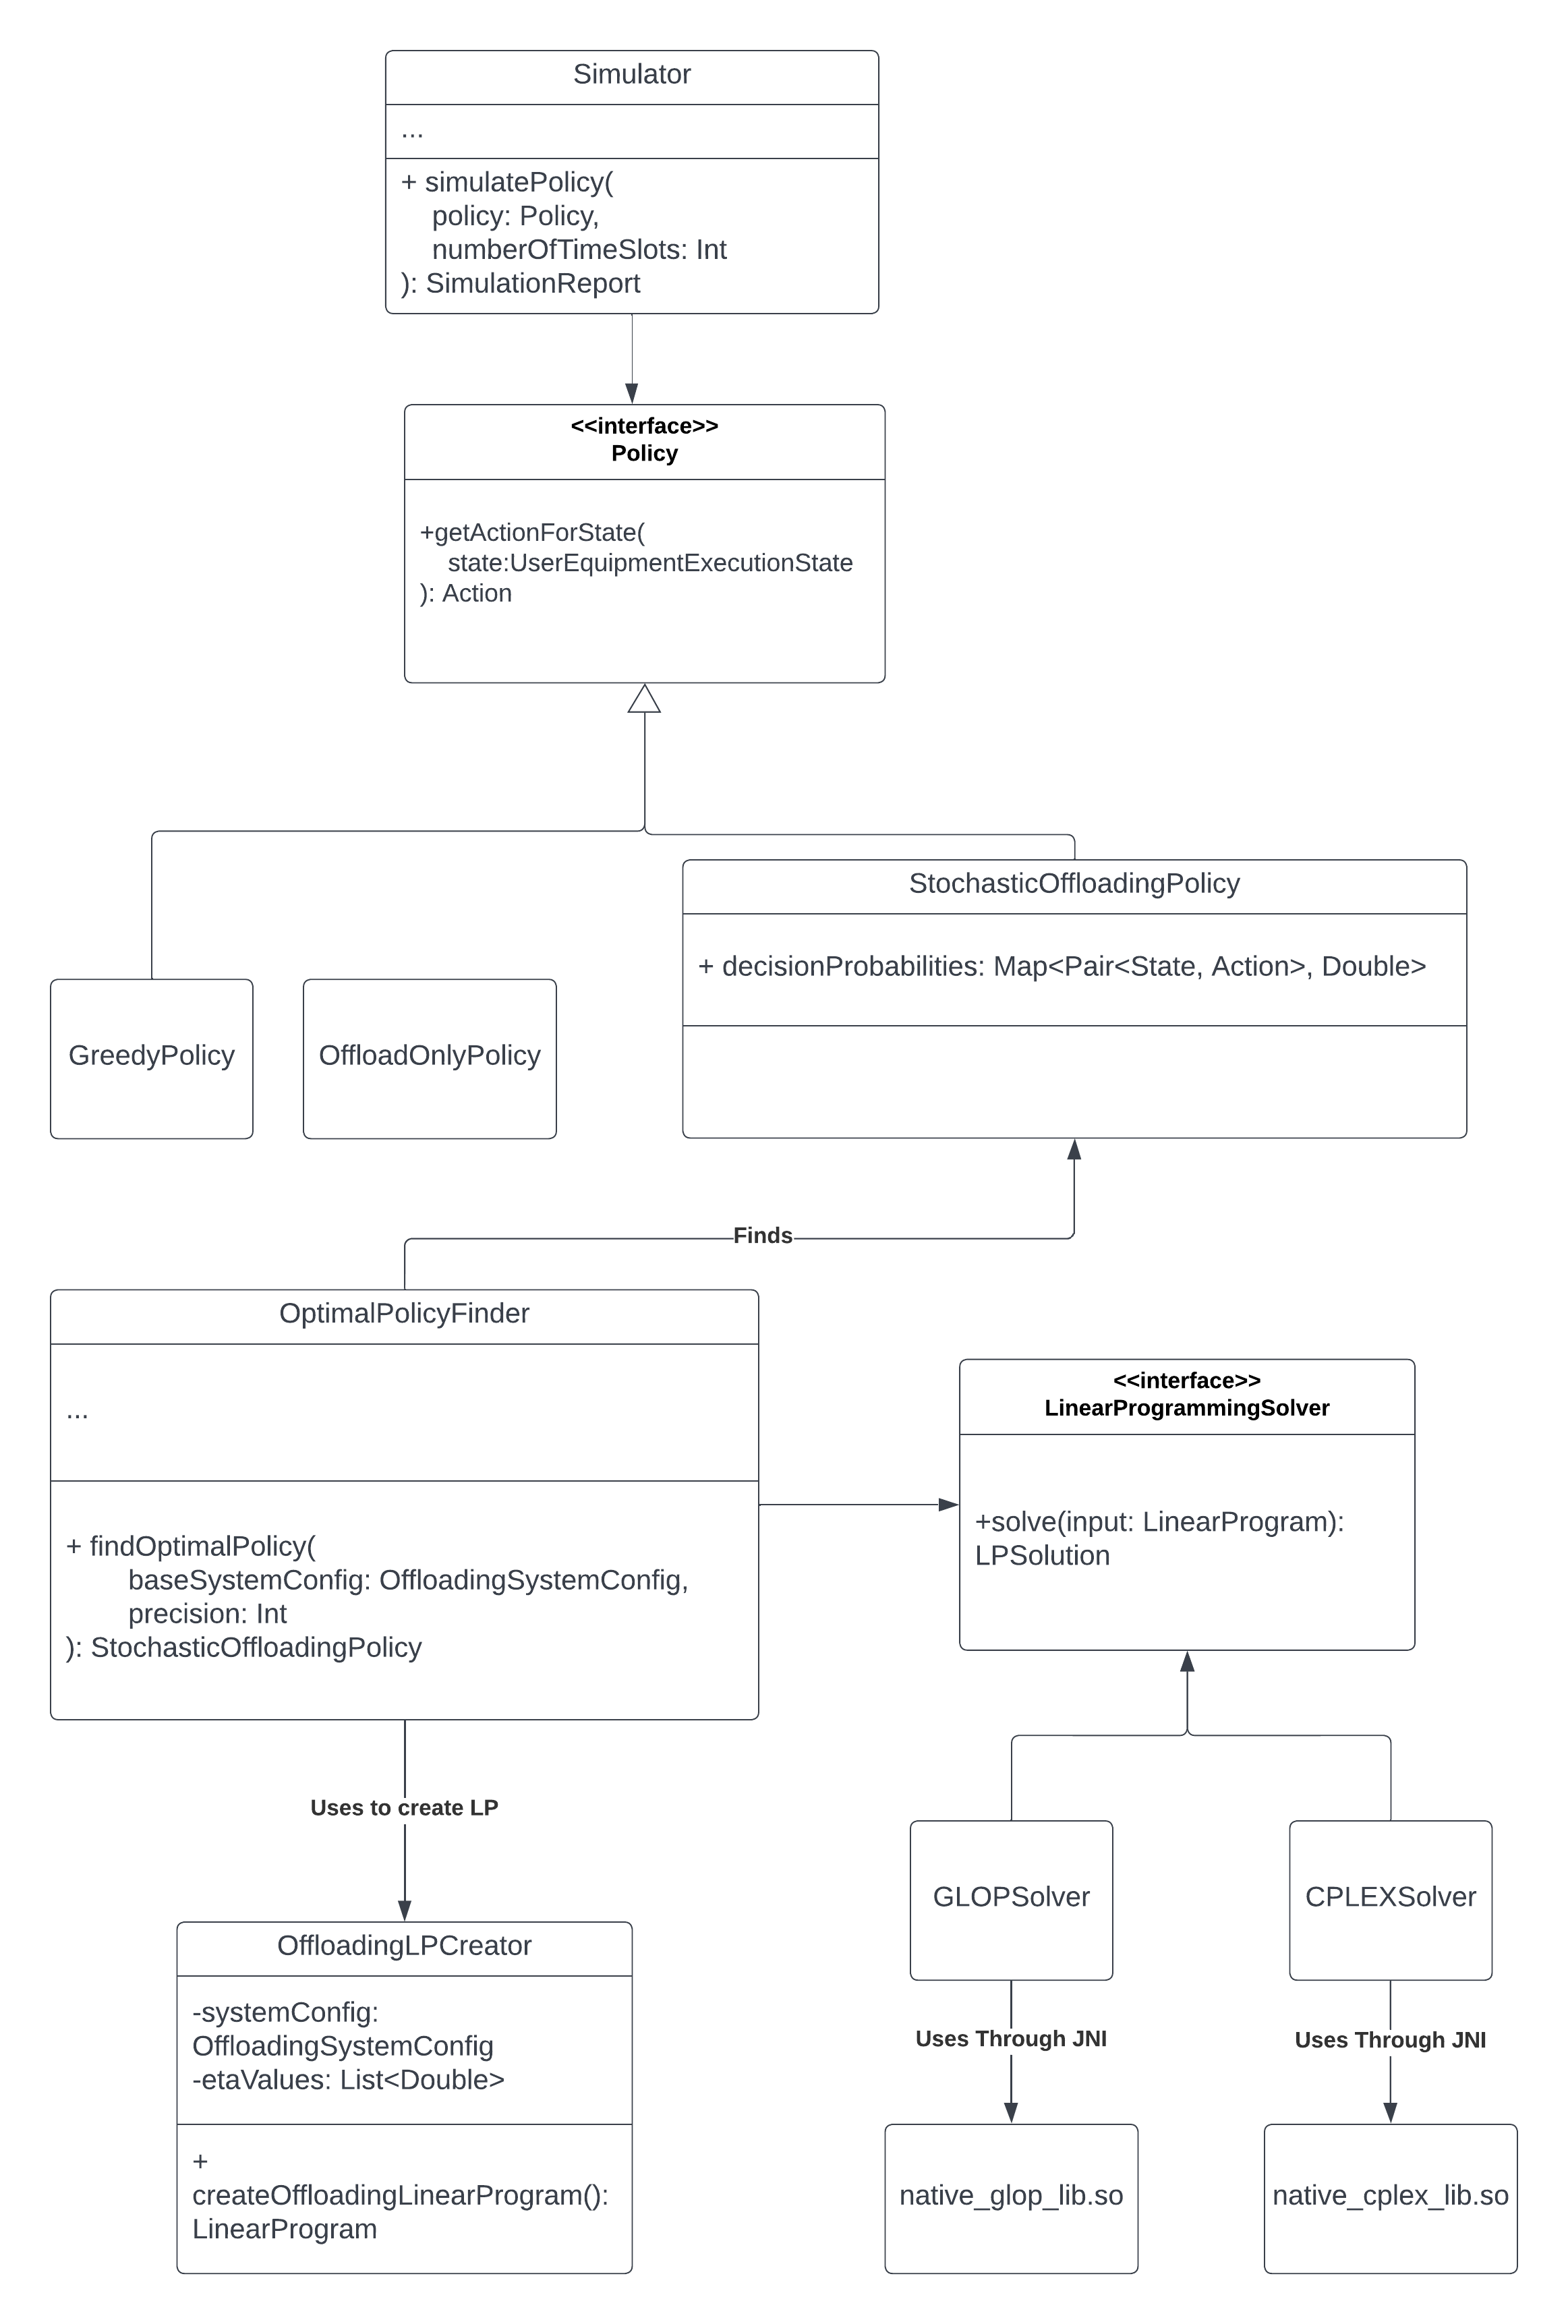
\includegraphics[width=0.8\textwidth]{cdiagram.png}
	\caption{کلاس دیاگرام چارچوب \lr{Kompute}}
	\label{fig:classdiagram}
\end{figure}
\section{مولفه‌های اصلی چارچوب \lr{Kompute}}
\subsection{واسط \lr{Policy}}
واسط \texttt{\footnotesize Policy} قردادی است که تمام استراتژی‌های تخلیه‌ی وظیفه باید آن را پیاده‌سازی کنند. همانطور که در فصل ۴ گفته شد، یک استراتژی تخلیه‌ی وظیفه، می‌بایست که با توجه به حالت سیستم در زمانی مشخص، تصمیم بگیرد که چه کنشی برای اجرا در آن بازه زمانی انتخاب شود. این منطق در کامپیوت با رابط مشخص‌شده در قطعه کد \ref{lst:policy} تعریف شده است.

\begin{LTR}
	\begin{lstlisting}[language=Kotlin, caption={واسط \lr{Policy}}, captiondirection=RTL, label={lst:policy}]
interface Policy {
	
	fun getActionForState(state: UserEquipmentExecutionState): Action
}
	\end{lstlisting}
\end{LTR}
به عنوان نمونه برای پیاده‌سازی استراتژی تخلیه‌ی وظیفه‌ی «حریصانه-تخلیه اول\LTRfootnote{Greedy-Offload First}» کلاس وارث مطابق با قطعه کد \ref{lst:greedy} تعریف می‌شود. این استراتژی تخلیه در صورتی که بتواند هم تخلیه و هم پردازش محلی انجام دهد، هر دو را انجام خواهد داد و در صورتی که تنها یک وظیفه در صف‌های وظایف باشد آن وظیفه را تخلیه خواهد کرد.
\begin{LTR}
	\begin{lstlisting}[language=Kotlin, caption={پیاده‌سازی استراتژی تخلیه‌ی وظیفه‌ی حریصانه-تخلیه‌ی اول}, captiondirection=RTL, label={lst:greedy}]
class GreedyOffloadFirstPolicy : Policy {
	
	override fun getActionForStateGreedy(state: UserEquipmentExecutionState): Action {
		if (state.averagePower() > state.pMax) return Action.NoOperation
		if (state.ueState.isCPUActive() && state.ueState.isTUActive()) {
			return Action.NoOperation
		}
		if (state.taskQueueLength.all { it == 0 }) return Action.NoOperation
		if (state.ueState.isCPUActive()) {
			return OffloadOnlyPolicy.getActionForState(state)
		}
		if (state.ueState.isTUActive()) {
			return LocalOnlyPolicy.getActionForState(state)
		}
		val nonEmptyIndices = state.taskQueueLength.indices.filter {
			state.taskQueueLength[it] > 0
		}
		require(nonEmptyIndices.isNotEmpty())
		val queueIndices: Pair<Int, Int>? = 
		state.ueState.getTwoRandomQueueIndicesForTwoTasks()
		if (queueIndices == null) {
			return Action.AddToTransmissionUnit(nonEmptyIndices[0])
		} else {
			return Action.AddToBothUnits(queueIndices.first, queueIndices.second)
		}
	}
}
	\end{lstlisting}
\end{LTR}
\subsection{کلاس \lr{OffloadingLPCreator}}
این کلاس وظیفه‌ی ساخت مسئله‌ی برنامه‌ریزی خطی
$\mathcal{P}_2$
که در رابطه‌ی \ref{eq:p2} بیان شد را دارد. بدین منظور این کلاس پنج شگرد زیر را تعریف می‌کند:
\begin{latin}
	\begin{itemize}
		\item \texttt{\footnotesize fun getObjectiveEquation(): EquationRow}
		\item \texttt{\footnotesize fun getEquation2(): EquationRow}
		\item \texttt{\footnotesize fun getEquations3(): List<EquationRow>}
		\item \texttt{\footnotesize fun getEquation4s(): List<EquationRow>}
		\item \texttt{\footnotesize fun getEquation5(): EquationRow}
	\end{itemize}
\end{latin}
که به ترتیب تابع هدف مسئله‌ی بهینه‌سازی و چهار شرط ذکر شده در \ref{eq:p2} را محاسبه می‌کنند. در نهایت با ترکیب این پنج تابع یک شی برنامه خطی توسط شگرد \texttt{\footnotesize createOffloadingLinearProgram} ایجاد می‌شود که به منظور محاسبه‌ی استراتژی تخلیه‌ی بهینه نیاز داریم که آن را حل کنیم. در ادامه به نحوه‌ی حل این برنامه خطی توسط کلاس‌های \texttt{\footnotesize Solver} می‌پردازیم.
\subsection{حل‌کننده‌ی خطی}
مولفه‌های شرکت‌کننده در حل مسئله‌ی بهینه‌سازی در کامپیوت، در شکل \ref{fig:solverdiagram} مشخص شده اند. در پایین‌ترین لایه برای حل مسئله برنامه‌ریزی خطی از حل‌کننده خطی به نام \lr{GLOP} استفاده شده است. این حل‌کننده جزئی از پروژه متن‌باز \lr{OR-Tools} است\LTRfootnote{\href{https://github.com/google/or-tools}{https://github.com/google/or-tools}} که توسط شرکت گوگل ارائه‌شده و نگه‌داری می‌شود. \Cite{glop} این حل‌کننده مانند اکثر حل‌کننده‌های سریع و مدرن، در زبان \lr{C++} نوشته شده است، اما احاطه‌گرهای آن در زبان‌های دیگر مانند پایتون، جاوا، و سی شارپ وجود دارد. در \CurrentProject، ما از احاطه‌گر زبان جاوا استفاده کرده‌ایم که در پروژه \lr{OR-Tools} با استفاده از رابط بومی جاوا و در قالب کلاس \texttt{\footnotesize MPSolver} پیاده‌سازی شده است. \\

در \lr{Kompute} کلاسی به نام \lr{GLOPSolver} وجود دارد که با گرفتن یک شی از نوع برنامه خطی در دامنه \lr{Kompute}، آن شی را به برنامه‌خطی قابل شناسایی برای کلاس \lr{MPSolver} تبدیل می‌کند و در نهایت نتیجه حل برنامه‌خطی را بر می‌گرداند. کلاس \lr{MPSolver} قابلیت پشتیبانی از برخی از حل‌کننده‌های دیگر به جز \lr{GLOP} را نیز دارد. با این وجود، به دلیل متن‌باز بودن پروژه، از برخی از حل‌کننده‌های تجاری معروف مانند \lr{CPLEX}\LTRfootnote{https://www.ibm.com/analytics/cplex-optimizer} پشتیبانی نمی‌کند. معماری \lr{Kompute} به گونه‌ای طراحی شده است که امکان استفاده از هر حل‌کننده‌ خطی در آن وجود داشته باشد. برای نمونه علاوه بر حل‌کننده پیش‌فرض \lr{GLOPSolver} کلاسی با نام \lr{CPLEXSolver} نیز در پروژه وجود دارد که در صورتی که نسخه تجاری \lr{CPLEX} که دارای جواز معتبر باشد بر روی سیستم کاربر نصب باشد از آن حل‌کننده استفاده خواهد شد.
\begin{figure}
	\centering
	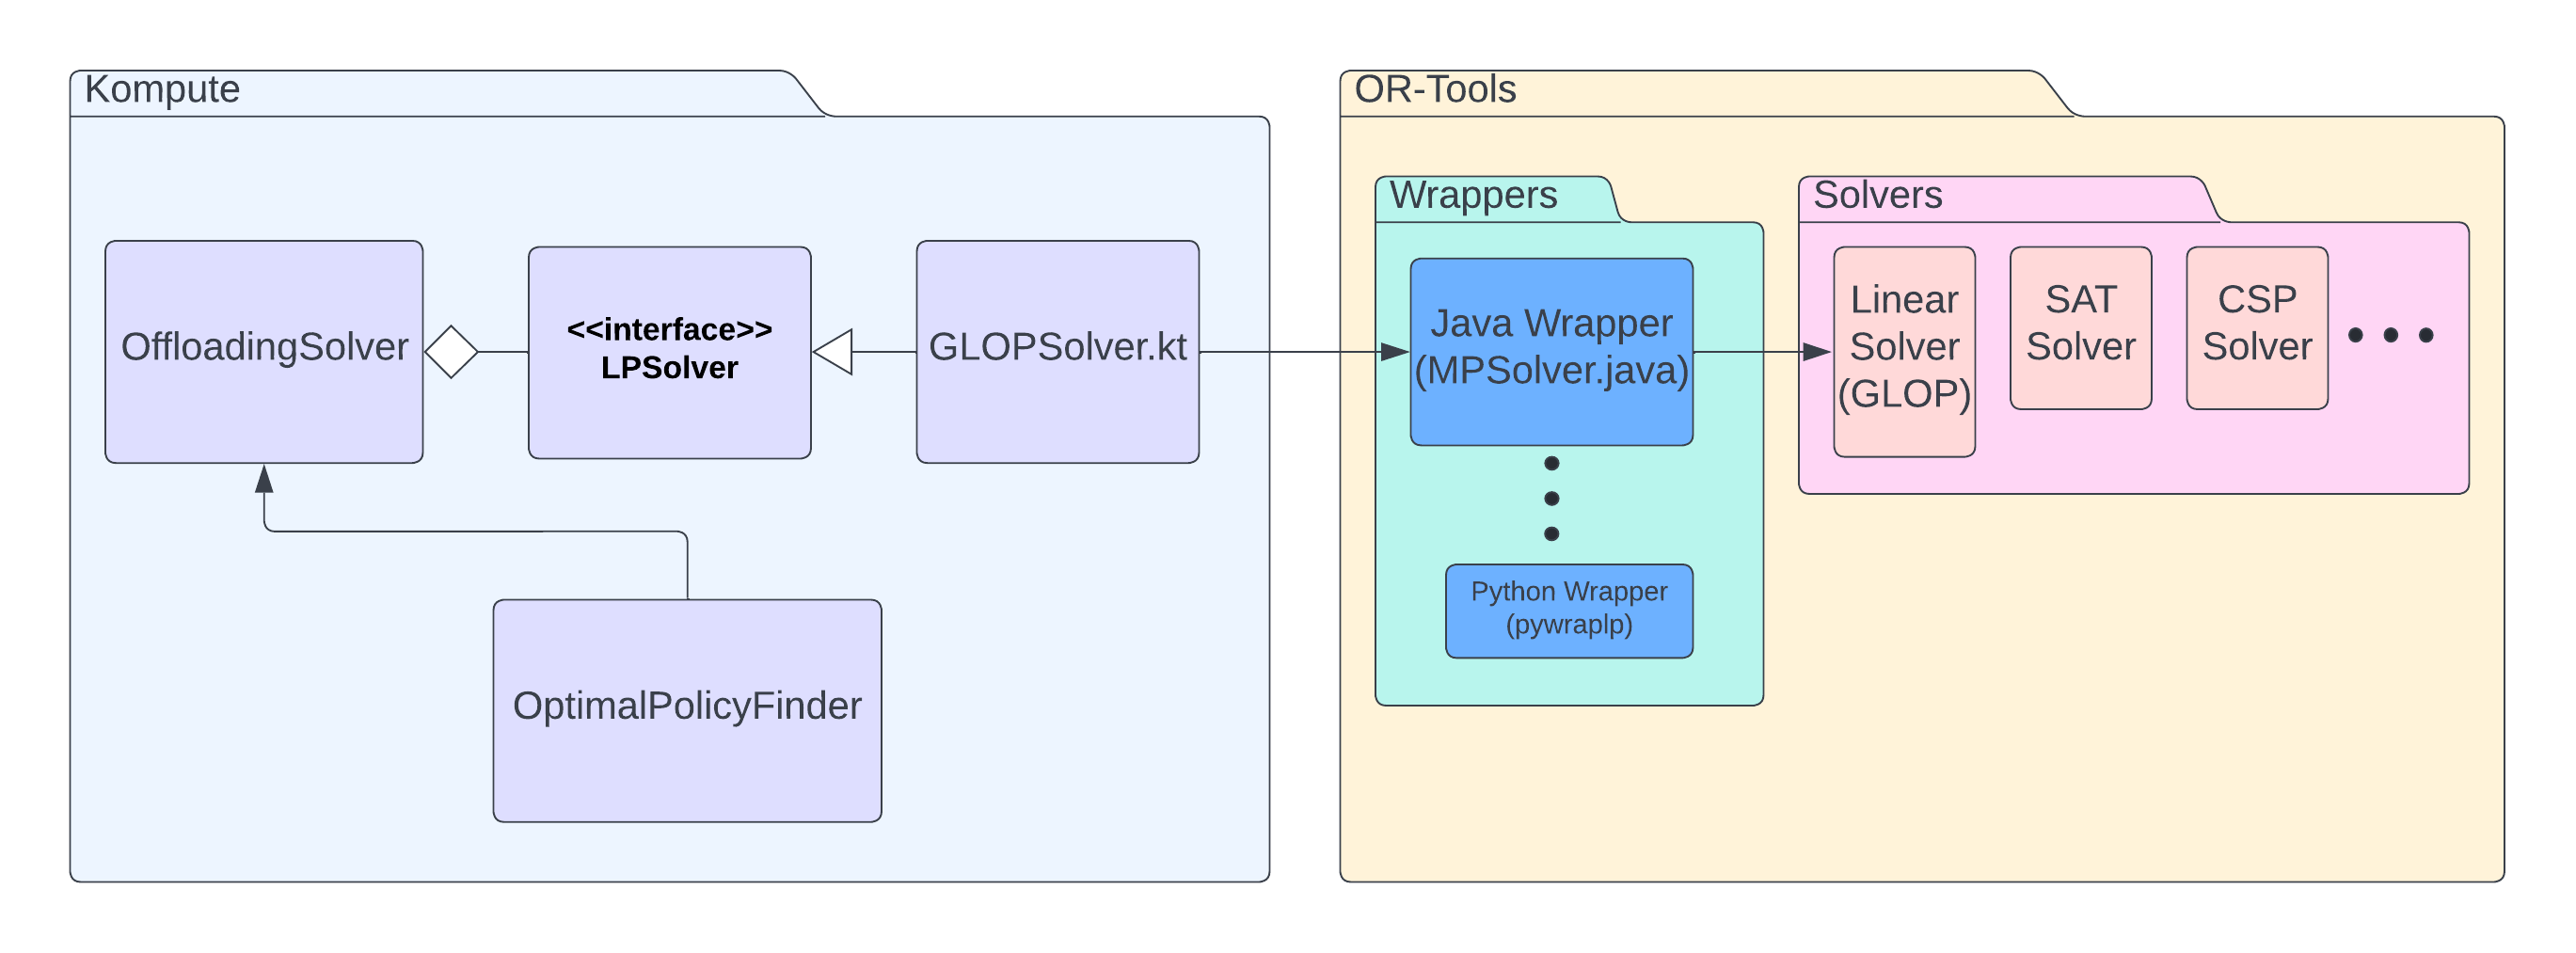
\includegraphics[width=\textwidth]{figures/solverdiagram.png}
	\caption{مولفه‌های شرکت‌کننده در حل مسئله‌ی بهینه‌سازی در \lr{Kompute}}
	\label{fig:solverdiagram}
\end{figure}
\newpage
\section{تعریف و حل یک مسئله‌ی تخلیه‌ی وظیفه‌ی نمونه در \lr{Kompute}}
در قطعه کد نمونه‌ی زیر، مسئله‌ی تخلیه‌ی وظیفه‌ برای محیط رایانش لبه‌ای با دو صف با نوع وظایف «سبک» و «سنگین» حل شده است.
\begin{LTR}
	\begin{lstlisting}[language=Kotlin, caption={تعریف و حل مسئله‌ی نمونه}, captiondirection=RTL, label={lst:solve}]
fun main(args: Array<String>) {
	val systemConfig = OffloadingSystemConfig(
		userEquipmentConfig = UserEquipmentConfig(
			stateConfig = UserEquipmentStateConfig(
				taskQueueCapacity = 5,
				tuNumberOfPackets = listOf(1, 3),
				cpuNumberOfSections = listOf(7, 2),
				numberOfQueues = 2
			),
			componentsConfig = UserEquipmentComponentsConfig(
				alpha = listOf(0.4, 0.9),
				beta = 0.90,
				etaConfig = null,
				pTx = 1.0,
				pLocal = 0.8,
				pMax = 1.7
			)
		),
		environmentParameters = EnvironmentParameters(
			nCloud = listOf(1, 1),
			tRx = 0.5,
		)
	)
	val optimalPolicy = RangedOptimalPolicyFinder.findOptimalPolicy(
		baseSystemConfig = systemConfig, 
		precision = 10
	)
	/*
	// For multi-threaded execution use this instead:
	val optimalPolicy = ConcurrentRangedOptimalPolicyFinder(
		baseSystemConfig = systemConfig
	).findOptimalPolicy(precision = 10, numberOfThreads = 8)
	*/
	val decisionProbabilities: Map<StateAction, Double>
		= optimalPolicy.stochasticPolicyConfig.decisionProbabilities
	println(decisionProbabilities)
}
	\end{lstlisting}
\end{LTR}
به این منظور ابتدا پارامترهای محیط تخلیه‌ی وظیفه در رایانش لبه‌ای را با استفاده از کلاس\linebreak \texttt{\footnotesize OffloadingSystemConfig} مشخص می‌کنیم. سپس استراتژی بهینه را با استفاده از کلاس \texttt{\footnotesize RangedOptimalPolicyFinder} با دقت لازم پیدا می‌کنیم. در نهایت جواب خروجی به صورت توزیع احتمالی بر روی مجموعه‌ی $|S| \times |A|$ بدست می‌آید.
\newpage
\section{نحوه‌ی شبیه‌سازی استراتژی‌های تخلیه‌ی وظیفه}
در قطعه کد نمونه‌ی زیر، استراتژی تخلیه‌ی بهینه و سه استراتژی تخلیه‌ی پایه شبیه‌سازی شده‌اند و نتایج تاخیر و توان مصرفی گزارش شده است.
\begin{LTR}
	\begin{lstlisting}[language=Kotlin, caption={شبیه‌سازی استراتژی‌های تخلیه‌ی وظیفه}, captiondirection=RTL, label={lst:sim}, showstringspaces=false]
fun main(args: Array<String>) {
	val baseSystemConfig: OffloadingSystemConfig = Mock.doubleQueueConfig()
	val alpha0Start = 0.01
	val alpha0End = 0.60
	val sampleCount = 30
	val simulationCycles = 1_000_000
	for (i in 0 until sampleCount) {
		val alpha0 = (alpha0Start + i * ((alpha0End - alpha0Start) / (sampleCount - 1)))
		val systemConfig = baseSystemConfig.withAlpha(0, alpha0)
		val optimalPolicy = RangedOptimalPolicyFinder.findOptimalPolicy(
			baseSystemConfig = systemConfig,
			precision = 10
		)
		val simulator = Simulator(systemConfig)
		val simulationResults = with(simulator) {
			listOf(
				simulatePolicy(LocalOnlyPolicy, simulationCycles),
				simulatePolicy(OffloadOnlyPolicy, simulationCycles),
				simulatePolicy(GreedyLocalFirstPolicy, simulationCycles),
				simulatePolicy(optimalPolicy, simulationCycles)
			)
		}
		val (localOnlyDelay,
			offloadOnlyDelay,
			greedyLocalFirstDelay,
			optimalDelay) = simulationResults.map { it.averageDelay }
		val (localOnlyAveragePower,
			offloadOnlyAveragePower,
			greedyLocalFirstAveragePower,
			optimalAveragePower) = simulationResults.map { it.averagePowerConsumption }
		println("$localOnlyDelay | " +
			"$offloadOnlyDelay | " +
			"$greedyLocalFirstDelay | " +
			"$optimalDelay")
		println("$localOnlyAveragePower | " +
			"$offloadOnlyAveragePower | " +
			"$greedyLocalFirstAveragePower | " +
			"$optimalAveragePower")
	}
}
	\end{lstlisting}
\end{LTR}
در این مثال به ازای مقادیر نرخ ورود مختلف برای صف شماره یک، با کمک کلاس \texttt{\footnotesize Simulator} معیارهای توان مصرفی و تاخیر محاسبه و گزارش شده است. پارامتر \texttt{\footnotesize simulationCycles} تعداد بازه‌های زمانی شبیه‌سازی را مشخص می‌کند. پرواضح است که هر چه این مقدار بالاتر باشد، دقت شبیه‌سازی بالاتر خواهد بود. 
\newpage